%%% -*- Coding: utf-8-unix; Mode: latex; TeX-master: "paper"; ispell-local-dictionary: "american" -*-

\section{Evolutionary and Co-Evolutionary Algorithms for Portfolio
  Optimization}
\label{sec:system}

All algorithms mentioned in this chapter are implemented to actually calculate the best possible portfolio throughout a specified time period which
forces them to adjust to changing market's conditions and provide the trading strategy as we can follow portfolio's composition adjustments made on a daily 
basis.  


\subsection{Genetic Algorithm}
\label{GA}

Genetic algorithms (GAs) are well-known and popular method of dealing with MOOPs.
They are described in great details in \cite{Mitchell01}.

Every time we try to use GAs to solve a problem we have to adjust it accordingly.
In our implementation each potential solution should be encoded inside a chromosome. 
Each chromosome represents portfolio composition (it is a normalized vector of double values representing percentage share of each stock).
Before first round of computation, the entire population is created from scratch using random values in chromosomes.

The following modified GA operations have been implemented:
\begin{description}
  \item [mutation]
      - mutation operator changes exactly one value $ \alpha_{i} $ representing percentage share of a specific stock $i$ (each time the value $i$ is chosen randomly)
      to $\alpha_{i}'$ ($\alpha_{i}' \in (0,1)$ is chosen randomly). 
      After that, we have to normalize the vector.
      \emph{Mutation\_coefficient} (\emph{mutation\_coefficient} $ \in (0,1)$ ) determines what part of the population will be subjected to mutation operator.
  \item [selection]
      - \emph{breeding\_coefficient} ( \emph{breeding\_coefficient} $ \in (0,1)$ ) determines what part of population will be subjected to crossover operator, selection is based on 
      fitness function (only the fittest part of the population will be selected);
  \item [crossover]
      - after selection chromosomes eligible for reproduction, each pair of chromosomes are subjected to crossover operator. As a result new chromosomes are created (each pair
      produces two new chromosomes) and added to population. Crossover choose points $left$  and $right$ (both are chosen randomly) which cut parent's chromosomes in the way
      presented in figure~\ref{fig:parents}. Children are created according to a process shown in figure~\ref{fig:children}.
      
       \begin{figure}[H]
	    \begin{center}
	      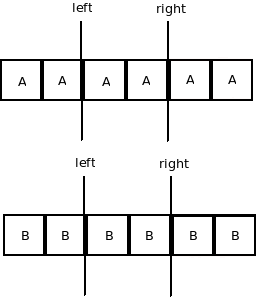
\includegraphics[scale=.3]{parents.png}
	    \end{center}
	    \caption{Example of parent's chromosomes split into 3 parts}
	    \label{fig:parents}
	  \end{figure}

	  \begin{figure}[H]
	    \begin{center}
	      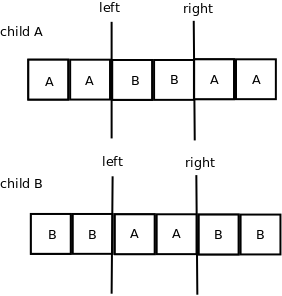
\includegraphics[scale=.3]{children.png}
	    \end{center}
	    \caption{Children's chromosomes contain mixed parent's genetic material}
	    \label{fig:children}
	  \end{figure}

\end{description}

Apart from that, extinction mechanism has been implemented.
At the end of each GA round a part of the population that has the lowest fitness is exterminated.
\emph{Extinction\_coefficient} determines what part of population will be subjected to extinction.
 
\subsubsection{Pseudocode}

Pseudocode of GA is presented in Algorithm~\ref{genetic_pseudo}.
We start by evaluating each chromosome using fitness function described in \ref{sec:gen_fitness_fun}, which uses current stock prices.
The fittest individuals are allowed to reproduce (this is further controlled by \emph{breeding\_coefficient}).
New individuals are merged to existing population.
After that, mutation is applied to a part of the least fit population to assure that population is diverse (in fact it is a way of implementing $reinitialization$
method, mentioned in \cite{zitz1999a}) and we do not miss any potentially better solutions.
Then we destroy some of the worst fit individuals which is useful because we can control the overall population size and we get rid of individual with chromosomes
not likely being successful in the future.
Finally, we return the best individual which becomes our trading strategy for next day (we adjust our current portfolio to the fittest individual solution). 


\begin{algorithm}
  \SetKwData{returnOrientedSubpopulation}{returnOrientedSubpopulation}
  \SetKwData{riskOrientedSubpopulation}{riskOrientedSubpopulation}
  \SetKwData{parents}{parents}
  \SetKwData{offspring}{offspring}
  \SetKwData{population}{population}
  \SetKwData{mutants}{mutants}
  \SetKwFunction{evaluate}{evaluate}
  \SetKwFunction{initialise}{initialise}
  \SetKwFunction{selectParents}{selectParents}
  \SetKwFunction{crossover}{crossover}
  \SetKwFunction{merge}{merge}
  \SetKwFunction{mutateLeastFitIndividuals}{mutateLeastFitIndividuals}
  \SetKwFunction{extinctLeastFitIndividuals}{extinctLeastFitIndividuals}
  \SetKwInOut{Input}{input}\SetKwInOut{Output}{output}
 
  \BlankLine
  \initialise{\population} \;
  
  \ForEach{$day$}{ 

      \ForEach{$individual$ $\in$ \population}{
	  \evaluate($individual$)\;
      }
     
      \parents $\leftarrow$  \selectParents{\population} \;
      \offspring $\leftarrow$ \crossover{\parents} \;
      \population  $\leftarrow$ \merge{\offspring, \population} \;

      \mutateLeastFitIndividuals{\population} \;

      \ForEach{$individual$ $\in$ \population}{
	  \evaluate($individual$)\;
      }

      \extinctLeastFitIndividuals{\population} \;
      \Return{the fittest individual} 
  }
  \caption{GA pseudocode}\label{genetic_pseudo}
\end{algorithm}




\subsubsection{Fitness function}
\label{sec:gen_fitness_fun}

Fitness is calculated according to the following formula (for portfolio with $N$ stocks):

\begin{equation}
    \gamma_{day} =  \sum_{i=1}^{N} {  \alpha_{i} * \frac{price(i,day)}{price(i,day - 1)} }
\end{equation}

where:

\begin{description}
  \item [$\gamma_{day}$] 
      is the value of the portfolio's fitness calculated for specific $day$;
  \item [$\alpha_{i}$]
      is the percentage share of a specific stock $i$ in the whole portfolio;
  \item [$price(i,day)$]
      returns the price of stock $i$ for a specific $day$.
\end{description}

Clearly, the fitness function favours the portfolios which have the highest day-to-day increase in value.
Of course such method of calculating fitness has many drawbacks e.g. it completely omits the aspect of risk associated with investing in highly volatile stocks.
However, it turns out that in spite of this obvious flaw the algorithm is performing quite well.  

\subsection{Co-evolutionary system}
\label{sec:co-evol-sys}

Contrary to \ref{GA}, in this approach two subpopulations coexist side by side.
Each individual represents potential solution to portfolio optimization problem.
Risk oriented subpopulation tries to optimize on risk (the lower risk value the better), whereas the return oriented subpopulation tries to maximize expected return.
Usually the greater the expected return the riskier the investment so our solutions will involve some trade-offs.
However that should not startle us, as we have already predicted in \ref{sec:multi} that optimization under such circumstances is not easy.

As presented in figure~\ref{fig:co-evol}, reproduction is allowed only between members of different subpopulations.
Not every member of a particular subpopulation is allowed to reproduce - only the fittest (fitness of a particular member depends on the subpopulation it belongs to - the fittest one
 in one subpopulation would probably be considered as one of the weakest in the other one).
Thanks to this approach the offspring that is created is very diverse.
In fact it is an application of $restricted$ $mating$ \cite{zitz1999a}.
Some part of the weakest members of both subpopulations is subjected to extinction.
Because of that we do not end up with too big population full of useless solutions.
In place of extinct members, offspring of the fittest is introduced to both subpopulations.

Apart from that, some members are subjected to mutations in order to even further maintain subpopulation diversity.
The migration mechanism has the same purpose - to avoid local extrema.
It is also described as an $isolation$ $by$ $distance$ \cite{zitz1999a}.
Risk as well as expected return are calculated according to Capital Asset Pricing Model (described in \cite{CAPM}) .
 

\begin{figure}[ht]  
	    \begin{center}
	      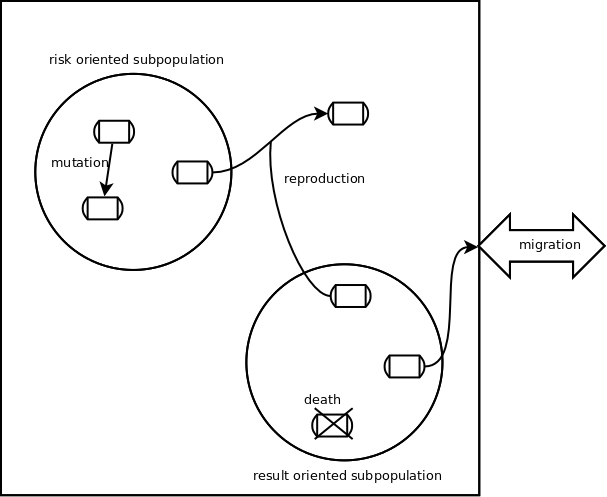
\includegraphics[scale=.2]{co-evol-2-sub.png}
	    \end{center}
	    \caption{Co-evolutionary system overview} 
	    \label{fig:co-evol}
	  \end{figure}

\subsubsection{Maintaining population diversity}

To sum up several mechanisms have been implemented to keep both subpopulations diverse:

\begin{itemize}
  \item crossover is allowed only between the fittest chromosomes from different subpopulations; 
  \item mutations introducing random genetic change;
  \item migration allows chromosomes to travel to different nodes.  
\end{itemize}

\subsubsection{Pseudocode}


\begin{algorithm}
  \SetKwData{returnOrientedSubpopulation}{returnOrientedSubpopulation}
  \SetKwData{riskOrientedSubpopulation}{riskOrientedSubpopulation}
  \SetKwData{parents}{parents}
  \SetKwData{offspring}{offspring}
  \SetKwData{population}{population}
  \SetKwData{mutants}{mutants}
  \SetKwFunction{evaluate}{evaluate}
  \SetKwFunction{initialise}{initialise}
  \SetKwFunction{selectParents}{selectParents}
  \SetKwFunction{recombine}{recombine}
  \SetKwFunction{merge}{merge}
  \SetKwFunction{mutateLeastFitIndividuals}{mutateLeastFitIndividuals}
  \SetKwFunction{extinctLeastFitIndividuals}{extinctLeastFitIndividuals}
  \SetKwInOut{Input}{input}\SetKwInOut{Output}{output}
 
  \BlankLine
  \initialise{\riskOrientedSubpopulation} \;
  \initialise{\returnOrientedSubpopulation} \;
  
  \ForEach{$day$}{ 

      \ForEach{$individual$ $\in$ \population}{
	  \evaluate($individual$)\;
      }
     
      \parents $\leftarrow$  \selectParents{\riskOrientedSubpopulation, \returnOrientedSubpopulation} \;
      \offspring $\leftarrow$ \recombine{\parents} \;
      \population  $\leftarrow$ \merge{\offspring, \riskOrientedSubpopulation, \returnOrientedSubpopulation} \;

      \mutateLeastFitIndividuals{\population} \;

      \ForEach{$individual$ $\in$ \population}{
	  \evaluate($individual$)\;
      }

      \extinctLeastFitIndividuals{\population} \;
      \Return{non-dominated solution} 
  }
  \caption{CEA pseudocode}\label{cea_pseudo}
\end{algorithm}

Contrary to GA, we are dealing with two populations (with different objectives) at once (see Algorithm~\ref{cea_pseudo}).
Apart from that, the pseudocode looks very similar.
Reproduction is only allowed between individuals from different subpopulations (which is a direct application of $restricted$ $mating$ method
 described in \cite{zitz1999a}).
To even further assure that populations remain diverse, we mutate part of the least fit individuals.
Extinction helps to control population size and get rid of useless individuals.
Non-dominated solution (in Pareto sense) is returned as a result.



\subsection{Co-Evolutionary Multi-agent System - CoEMAS}

Co-evolutionary Multi-agent System (CoEMAS) is the most sophisticated system that has been implemented.
As described in \cite{drezewski2008coevolutionary} and \cite{drezewski2008agent-based-cooperative} such systems need environment as well as a set of autonomous agents interacting with each other.
Potential solution to portfolio optimization problem is stored inside each agent.


\begin{figure}[ht]   
	    \begin{center}
	      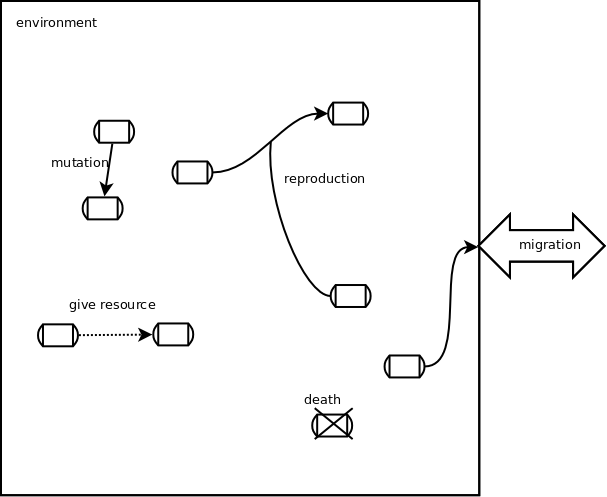
\includegraphics[scale=.2]{agent.png}
	    \end{center}
	    \caption{Overview of CoEMAS} 
	  \end{figure}

Contrary to \ref{sec:co-evol-sys} there are no subpopulations.
Instead of them we introduced individuals of two different species.
Each species focuses on different task:

\begin{itemize}
  \item species number 1 - tries to achieve the lowest risk possible;
  \item species number 2 - tries to achieve the highest expected return possible.
\end{itemize}

Risk as well as expected return is calculated due to Capital Asset Pricing Model (defined in \cite{CAPM}).

\subsubsection{Implemented actions}

Implemented actions that each agent can perform include:

\begin{description}
  \item [death]
      - if amount of resource that agent posseses is lower than threshold value the agent dies;
  \item [migration]
      - agent is allowed to migrate but the probability of this action is low;
  \item [reproduction]
      - agents from different species are allowed to reproduce provided that they both exceed the minimum amount of resource allowing to reproduce;
  \item [give/get]
      - agent can get resource from other, dominated agent;
  \item [recombination]
      - agents produce offspring by the means of recombination;
  \item [mutation]
      - mutation introduces random change to potential solution, normalization of solution vector is then required;
  \item [seek]
      - agents appropriate  to reproduction as well as get operation can be found thanks to this action.
\end{description}

Interactions between agents are implemented in the following way:
\begin{itemize}
  \item co-evolution is implemented as a sequence of \emph{turns};
  \item in each \emph{turn} every agent perform its action (action to perform at any particular turn is chosen with some well defined probability, e.g. there is a 10\% chance that agent will try to find
	a partner to reproduce, 60\% chance that the agent will try to get some resource from dominated agent);
  \item when every agent performed some action the \emph{turn} ends and entire population of agents is checked whether some of them should die (not enough resource left after other agents got resource
	from it).
\end{itemize}


Each agent performs one of the above actions with some probability.

\subsubsection{Pseudocode}


% \STATE randomly INITIALISE agents of two different species (risk oriented and return oriented) 
% \FORALL{ $day$ }
% 
%   \FOR{$round = 1$ $to$  $number\_of\_rounds$}  
%       \FORALL{ $agent$ $\in$ population }
%   \STATE choose a profile for $agent$
%   \STATE $agent$ should act according to a selected profile  
%       \ENDFOR
%   \ENDFOR
%   \RETURN non-dominated agent as a solution  
% \ENDFOR


\begin{algorithm}
  \SetKwData{Profile}{profile}\SetKwData{This}{this}\SetKwData{Up}{up}
  \SetKwFunction{Union}{Union}\SetKwFunction{chooseProfile}{chooseProfile}
  \SetKwInOut{Input}{input}\SetKwInOut{Output}{output}
 
  \BlankLine
  \emph{randomly INITIALISE agents of two different species (risk oriented and return oriented)}\;
  \ForEach{$day$}{ 

    \For{$round\leftarrow 1$ \KwTo $number\_of\_rounds$}{\label{forins}
      \ForEach{$agent$ $\in$ population}{
      
      \Profile$\leftarrow$ \chooseProfile{}\;

      \If(){\Profile is $resource\_profile$ }{\label{lt}
        perform actions specified in $resource\_profile$ 
      }

      \If(){\Profile is $reproduction\_profile$ }{\label{lt}
        perform actions specified in $reproduction\_profile$ 
      }

      \If(){\Profile is $migration\_profile$ }{\label{lt}
        perform actions specified in $migration\_profile$ 
      }
      
    }
}
  }
  \caption{CoEMAS pseudocode}\label{coemas_pseudo}
\end{algorithm}

Pseudocode of CoEMAS is presented in Algorithm~\ref{coemas_pseudo}.

Profiles are chosen with following probabilities:
\begin{itemize}
  \item $resource$ $profile$ - with probability 0.6;
  \item $reproduction$ $profile$ - with probability 0.2;
  \item $migration$ $profile$ with probability 0.1;
  \item $mutation$ $profile$ with probability 0.1.
\end{itemize}

Similarly to \ref{sec:co-evol-sys}, mutation is used as a mean of maintaining population diversity.
